\documentclass{beamer}
\usepackage{lipsum}

\mode<presentation>{\usetheme{Ringerike}}
\usepackage[english]{babel}
\usepackage[latin1]{inputenc}
\usepackage{multicol}

%\usepackage{amsmath,amsthm, amssymb, latexsym}
\boldmath
\usepackage[size=custom,width=150,height=85]{beamerposter}

\addtobeamertemplate{block begin}{}{\setlength{\parskip}{30pt plus 1pt minus 1pt}}
\setbeamertemplate{caption}[numbered]

\title{GEOSAT}
\subtitle{Combining VLBI, SLR, GNSS, and DORIS at the observation level}
\author{Per Helge Andersen, Michael D\"ahnn, Ingrid Fausk, Geir Arne Hjelle, Ann-Silje Kirkvik, Eirik Mysen}
\institute{Norwegian Mapping Authority, Geodetic Institute}
\date{April 15th, 2015}

\newlength{\techheight}
\setlength{\techheight}{8cm}
\usebackgroundtemplate{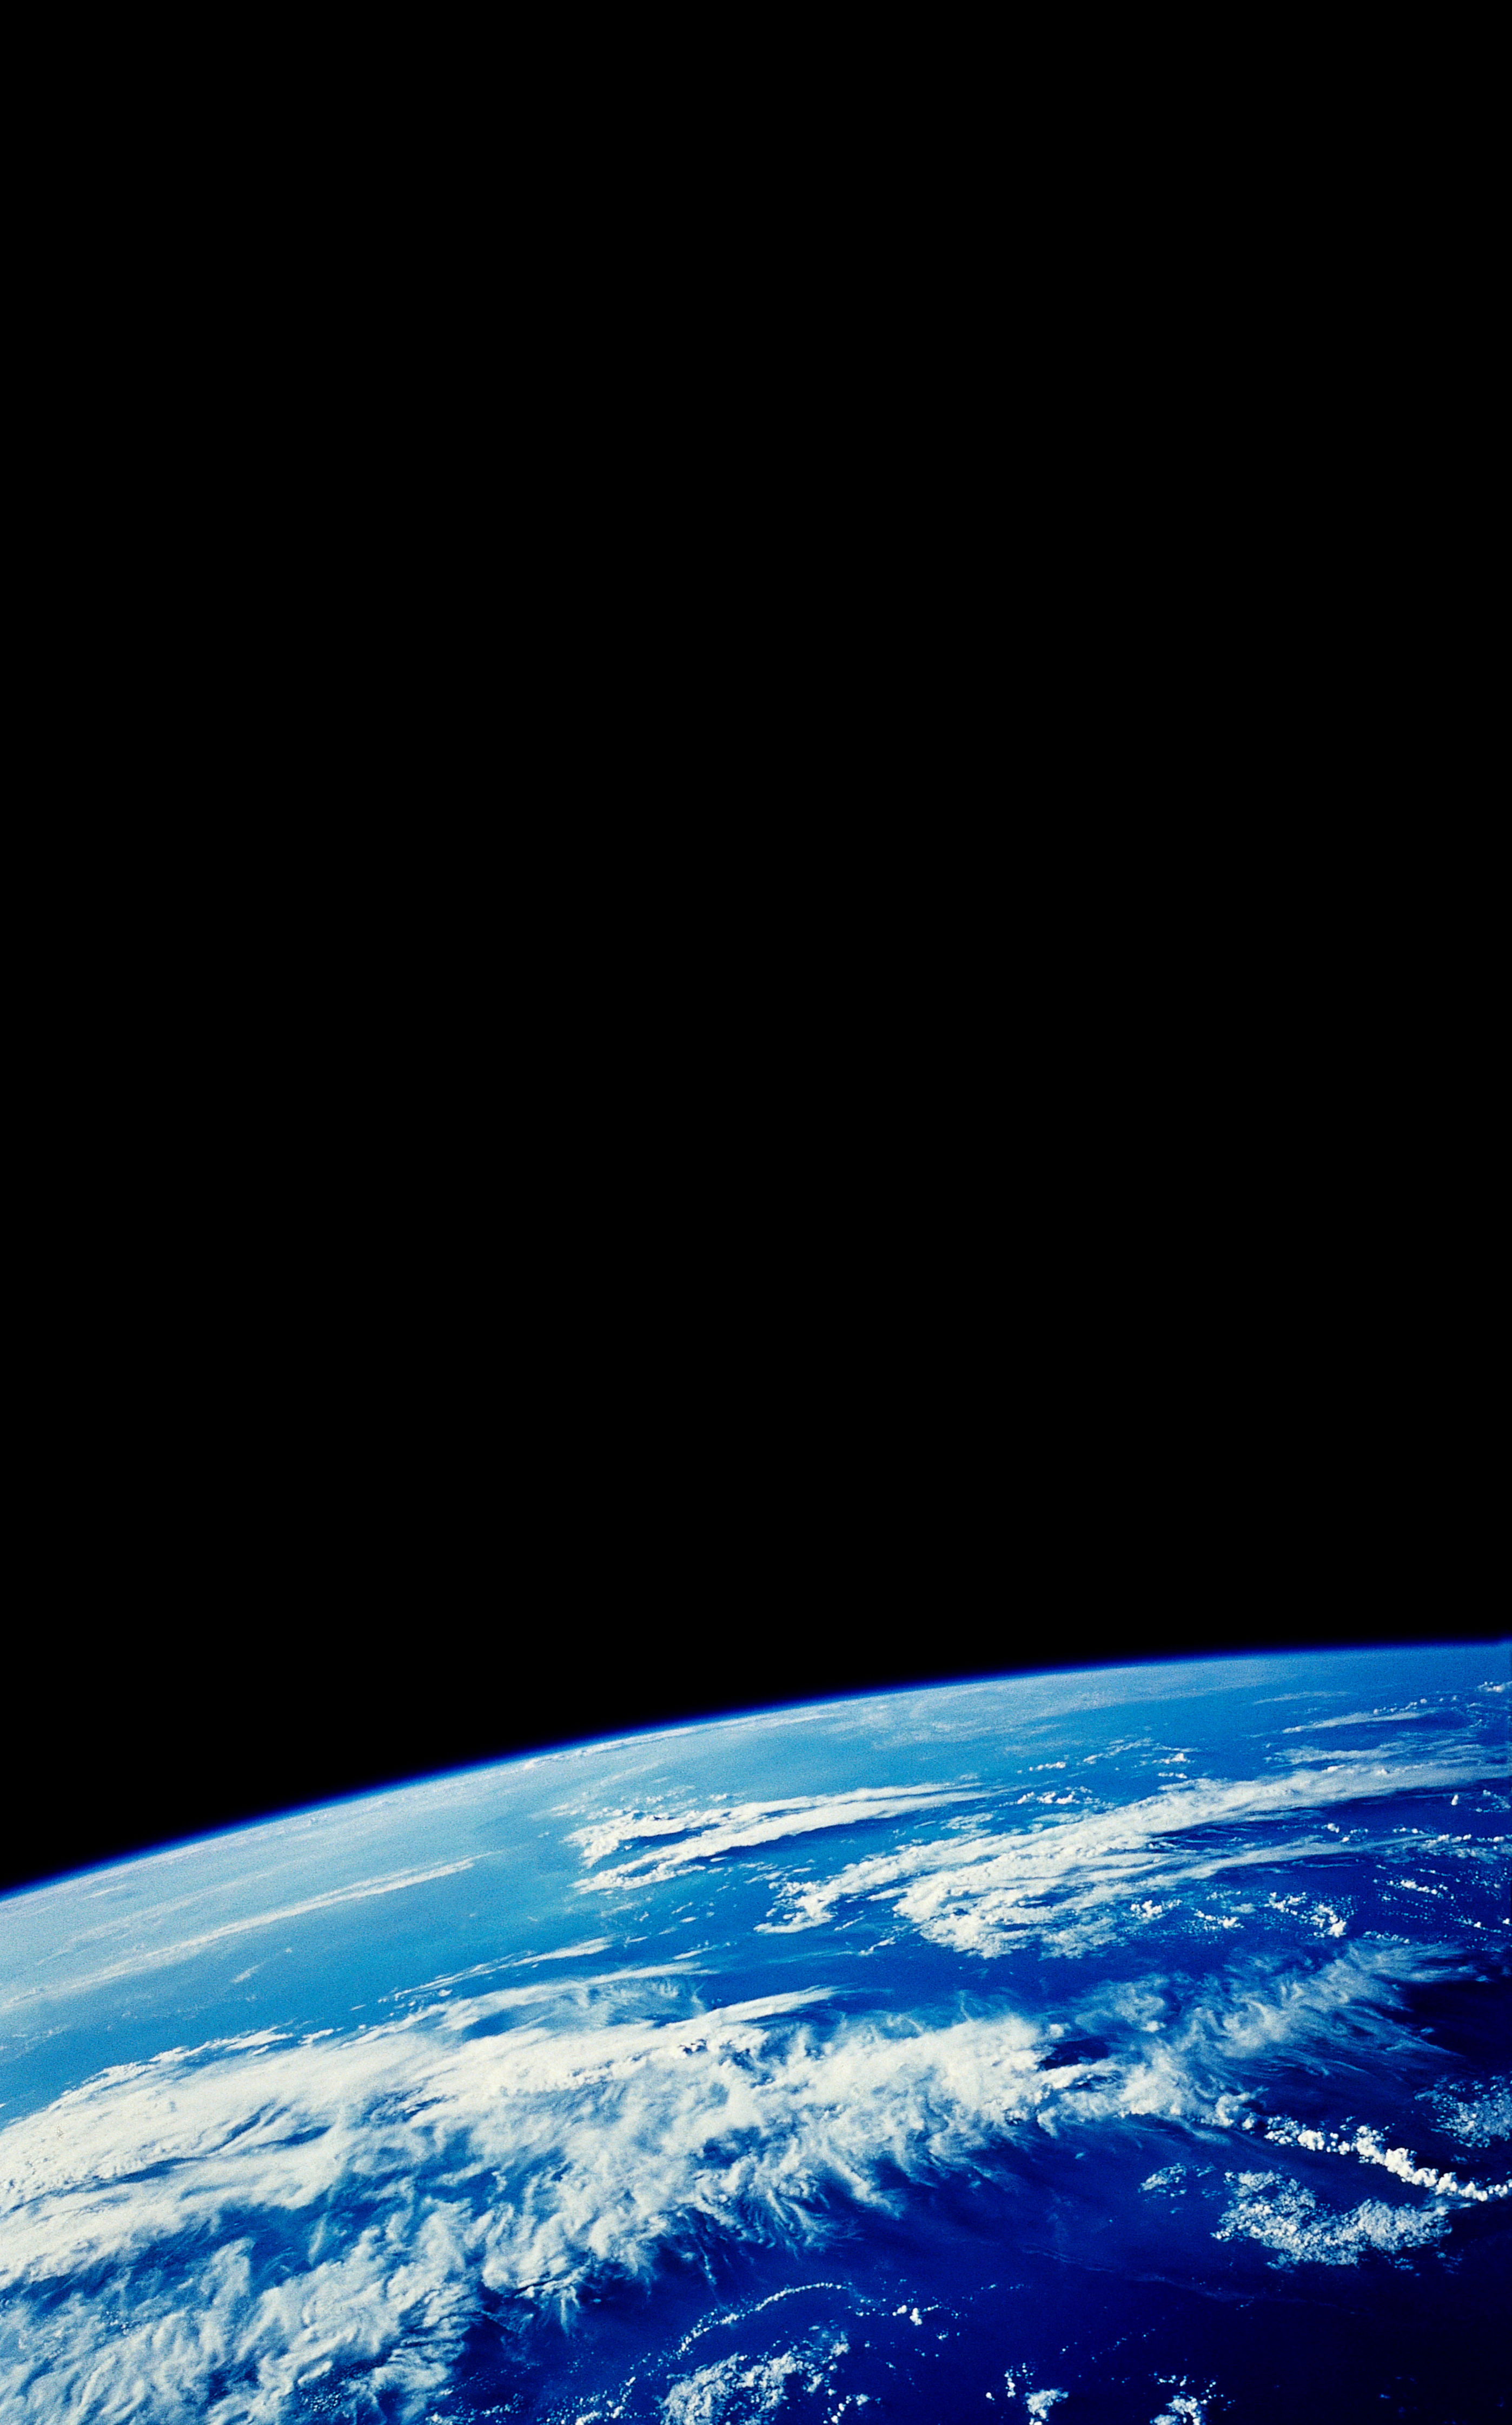
\includegraphics[height=\paperheight]{figure/earth}}

\begin{document}
\begin{frame}
  \begin{columns}
    \begin{column}{.32\textwidth}
      % Left title column
      \color{white} 
      \vspace*{2cm} \\
      {\bfseries\fontsize{250}{270}\selectfont\inserttitle}\\[3cm]
      {\fontsize{88}{120}\selectfont
        \insertsubtitle}\\[2cm]
      {\fontsize{45}{45}\selectfont
        \insertauthor\\[0.5cm]\itshape\insertinstitute}\\[3cm]

      {\fontsize{36}{42}\selectfont\setlength{\parskip}{36pt} At the Norwegian Mapping Authority, we are currently developing Where, a new
software for geodetic analysis. Where is built on our experiences with the
Geosat software, and will be able to analyse and combine data from VLBI, SLR,
GNSS and DORIS. The software is mainly written in Python which has proved very
fruitful. The code is quick to write and the architecture is easily extendable
and maintainable, while at the same time taking advantage of well-tested libraries
like the SOFA and IERS packages.

At the moment the VLBI analysis is close to ready. Comparison to other softwares
show that theoretical delay computations in Where are consistent with those. SLR
and GNSS analysis is well under way.

\vspace*{-10cm}

\endinput
}
      \raisebox{-26cm}{\kern43cm\color{white}\footnotesize
      PHOTO: GETTY IMAGES}
    \end{column}
    \begin{column}{.02\textwidth}
    \end{column}
    \begin{column}{.6\textwidth}
      % Content area
      \begin{columns}
        \begin{column}{.22\textwidth}
          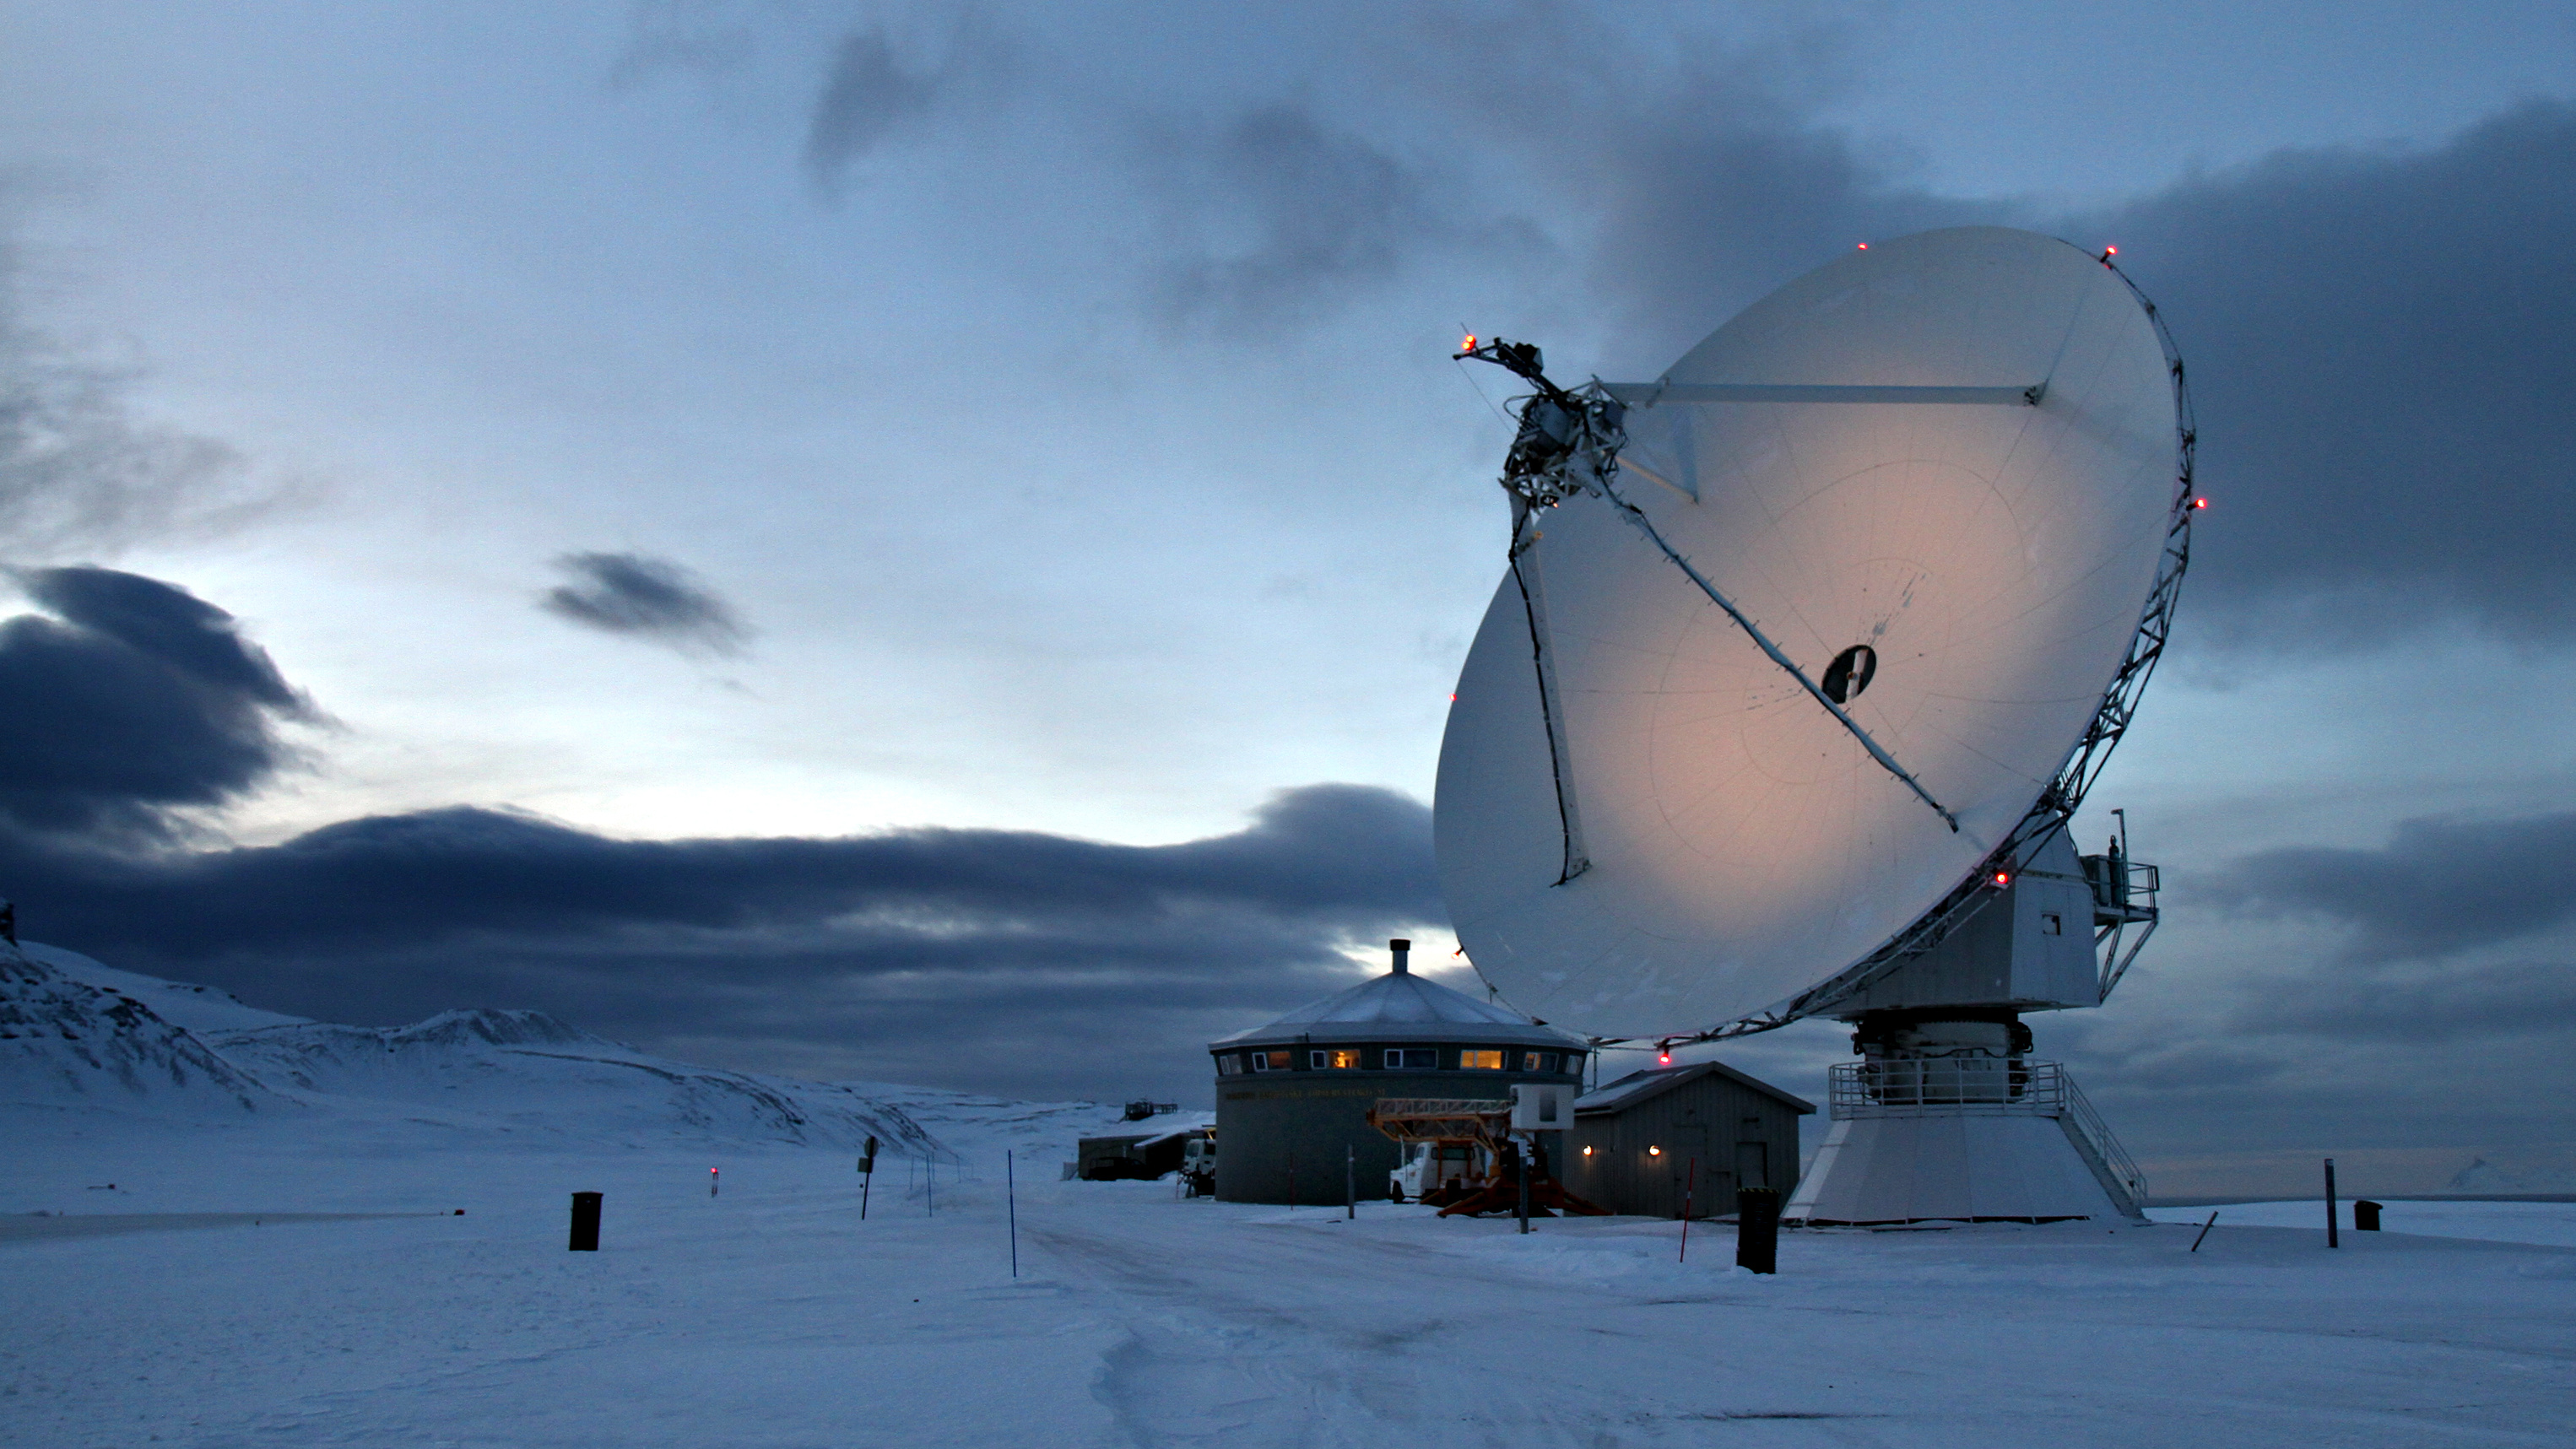
\includegraphics[width=\textwidth]{figure/vlbi}
          \raisebox{10cm}{\kern-19cm\tiny
            PHOTO: BJ�RN-OWE HOLMBERG}
          \vskip-1ex
          \begin{block}{VLBI}
            \vskip-3ex
            \parbox[t][\techheight]{0.95\textwidth}{\raggedrightVery Long Baseline Interferometry (VLBI) is a technique where several huge
telescopes collects signals from radio sources in space, e.g. quasars. By
comparing the arrival times of the signal at different telescopes we can
calculate the distance between the telescopes.

\endinput
}
          \end{block}
        \end{column}
        \begin{column}{.22\textwidth}
          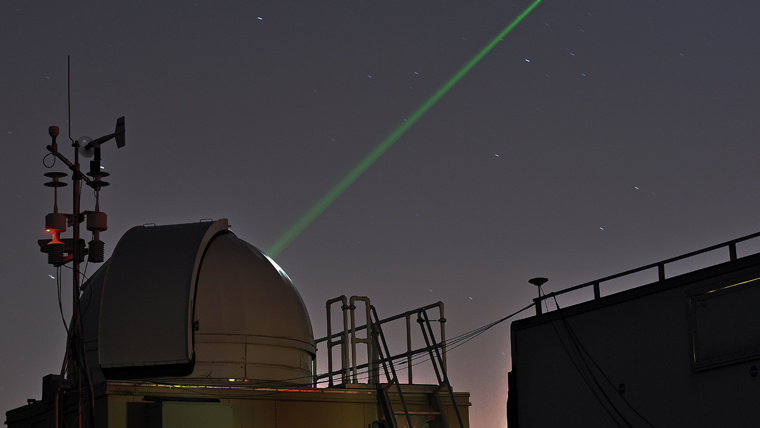
\includegraphics[width=\textwidth]{figure/slr}
          \raisebox{10cm}{\kern-6cm\color{white}\tiny
            PHOTO: FELIPE HALL / HTSI}
          \vskip-1ex
          \begin{block}{SLR}
            \vskip-3ex
            \parbox[t][\techheight]{0.95\textwidth}{\raggedright\documentclass[12pt,table,t]{beamer}

% Packages
\usepackage[norsk]{babel}
\usepackage[utf8]{inputenc}

% Theme
\mode<presentation>
{
  \usetheme{Honefoss}
  \setbeamertemplate{blocks}[rounded]
}

\newcommand{\comment}[1]{{\slshape\color{kvred}#1}}
\setbeamertemplate{caption}{\raggedright\insertcaption\par}

\title{Lasermålinger mot satellitter}
\subtitle{}
\author{Ingrid Fausk}
\date{Geodesi- og hydrografidagene, 27. november 2019}

\begin{document}
\frame[plain]{\titlepage}

\begin{frame}{Kartverkets ambisjoner innen SLR}
  \framesubtitle{Satellite Laser Ranging}
  \vspace{0.7cm}
  \begin{columns}
    \column{0.45\textwidth}
      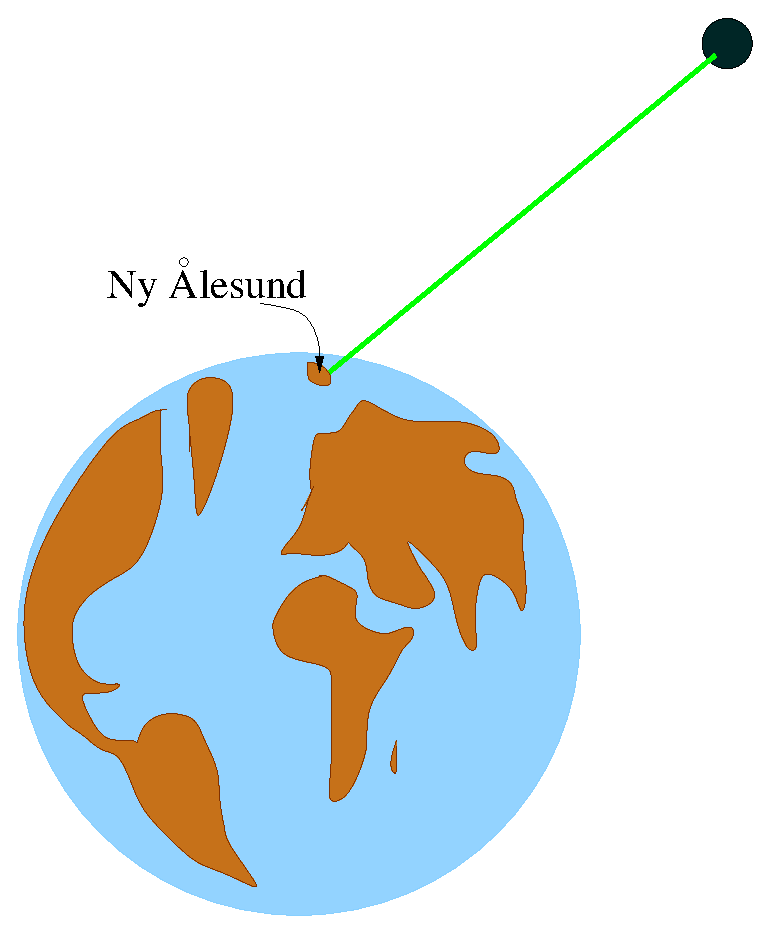
\includegraphics[width=0.95\textwidth]{figure/jordklode.eps}
    \column{0.45\textwidth}
      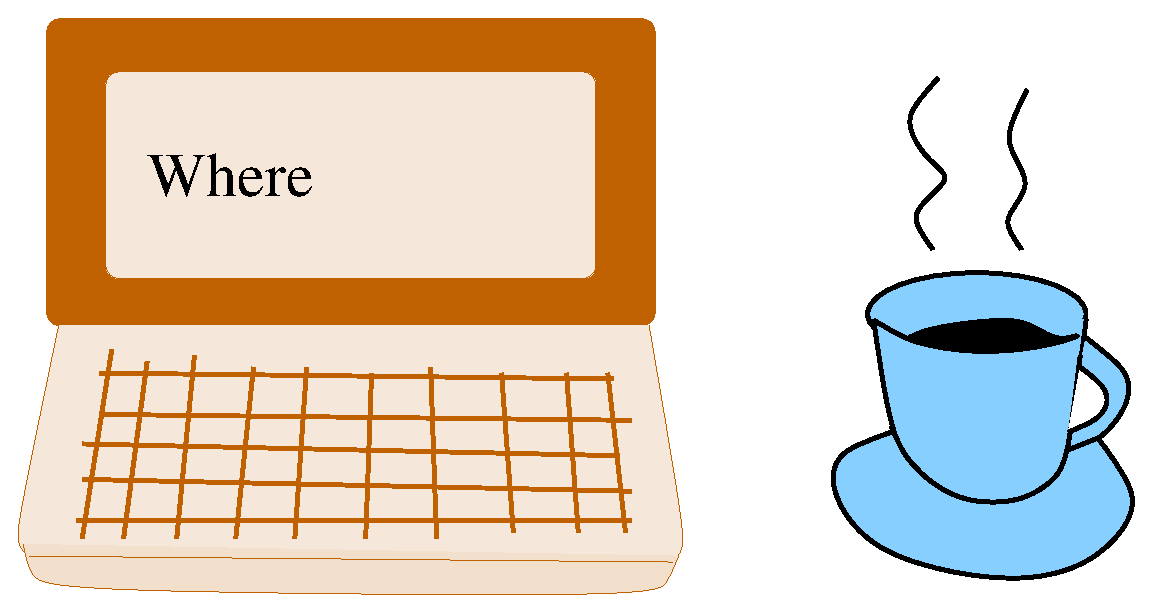
\includegraphics[width=0.95\textwidth]{figure/where.eps}
  \end{columns}
\end{frame}


\begin{frame}{Retroreflektorer}
  \begin{tabular}{cl}
    &  \\
    \raisebox{-.5\height}{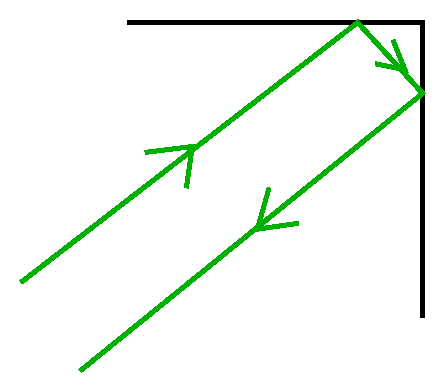
\includegraphics[width=0.2\textwidth]{figure/laser.eps}} & 
    \begin{minipage}[t]{0.6\columnwidth}Lyset reflekteres i samme retning som det kom fra \end{minipage}\\
    &  \\     
    \raisebox{-.5\height}{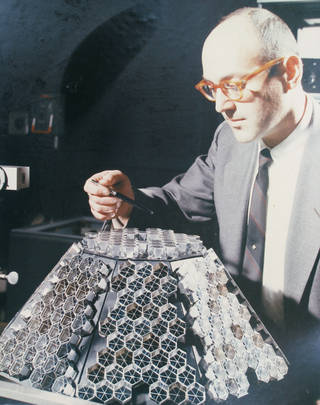
\includegraphics[width=0.2\textwidth]{figure/plotkin_-_beacon_explorer_a2.jpg}} & 
    \begin{minipage}[t]{0.6\columnwidth}Første satellitt med retroreflektorer, Beacon Explorer B, 1964. Henry Plotkin undersøker reflektorene.\end{minipage}\\
  \end{tabular}
\end{frame}


\begin{frame}{LAser GEOdynamics Satellite}
  \begin{columns}
    \column{0.6\textwidth}
      \begin{itemize}
        \item LAGEOS-1, 1976 (USA)
        \item LAGEOS-2, 1992 (Italia)
        \item Vekt: 400 kg
        \item Omløpstid: 220 min
        \item Høyde: 5800 km
        \item Diameter: 60 cm
        \item Levetid: 8.4 mill år. Inneholder en tidskapsel. 
      \end{itemize}
    \column{0.3\textwidth}
      \begin{figure}
        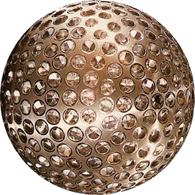
\includegraphics[width=0.7\textwidth]{figure/lageos_1.jpg} \caption{Photo: NASA}
      \end{figure}
  \end{columns}
\end{frame}


\begin{frame}{Stasjonsnettverk}
  \begin{figure}
    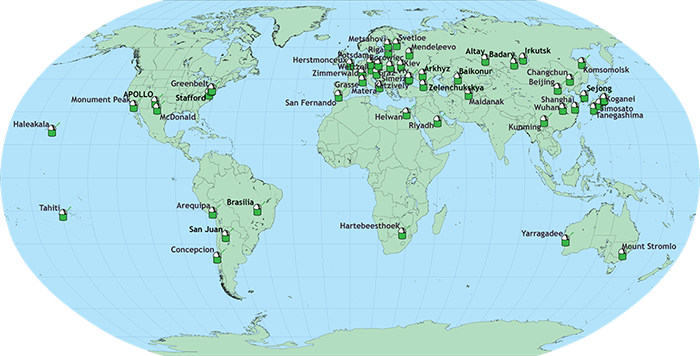
\includegraphics[width=0.9\textwidth]{figure/slrmap.png}\caption{Grafikk: NASA}
  \end{figure}
\end{frame}


\begin{frame}{Ny Ålesund}
  \framesubtitle{SLR ferdigstilles i 2024, bygges av NASA}
  \begin{figure}
    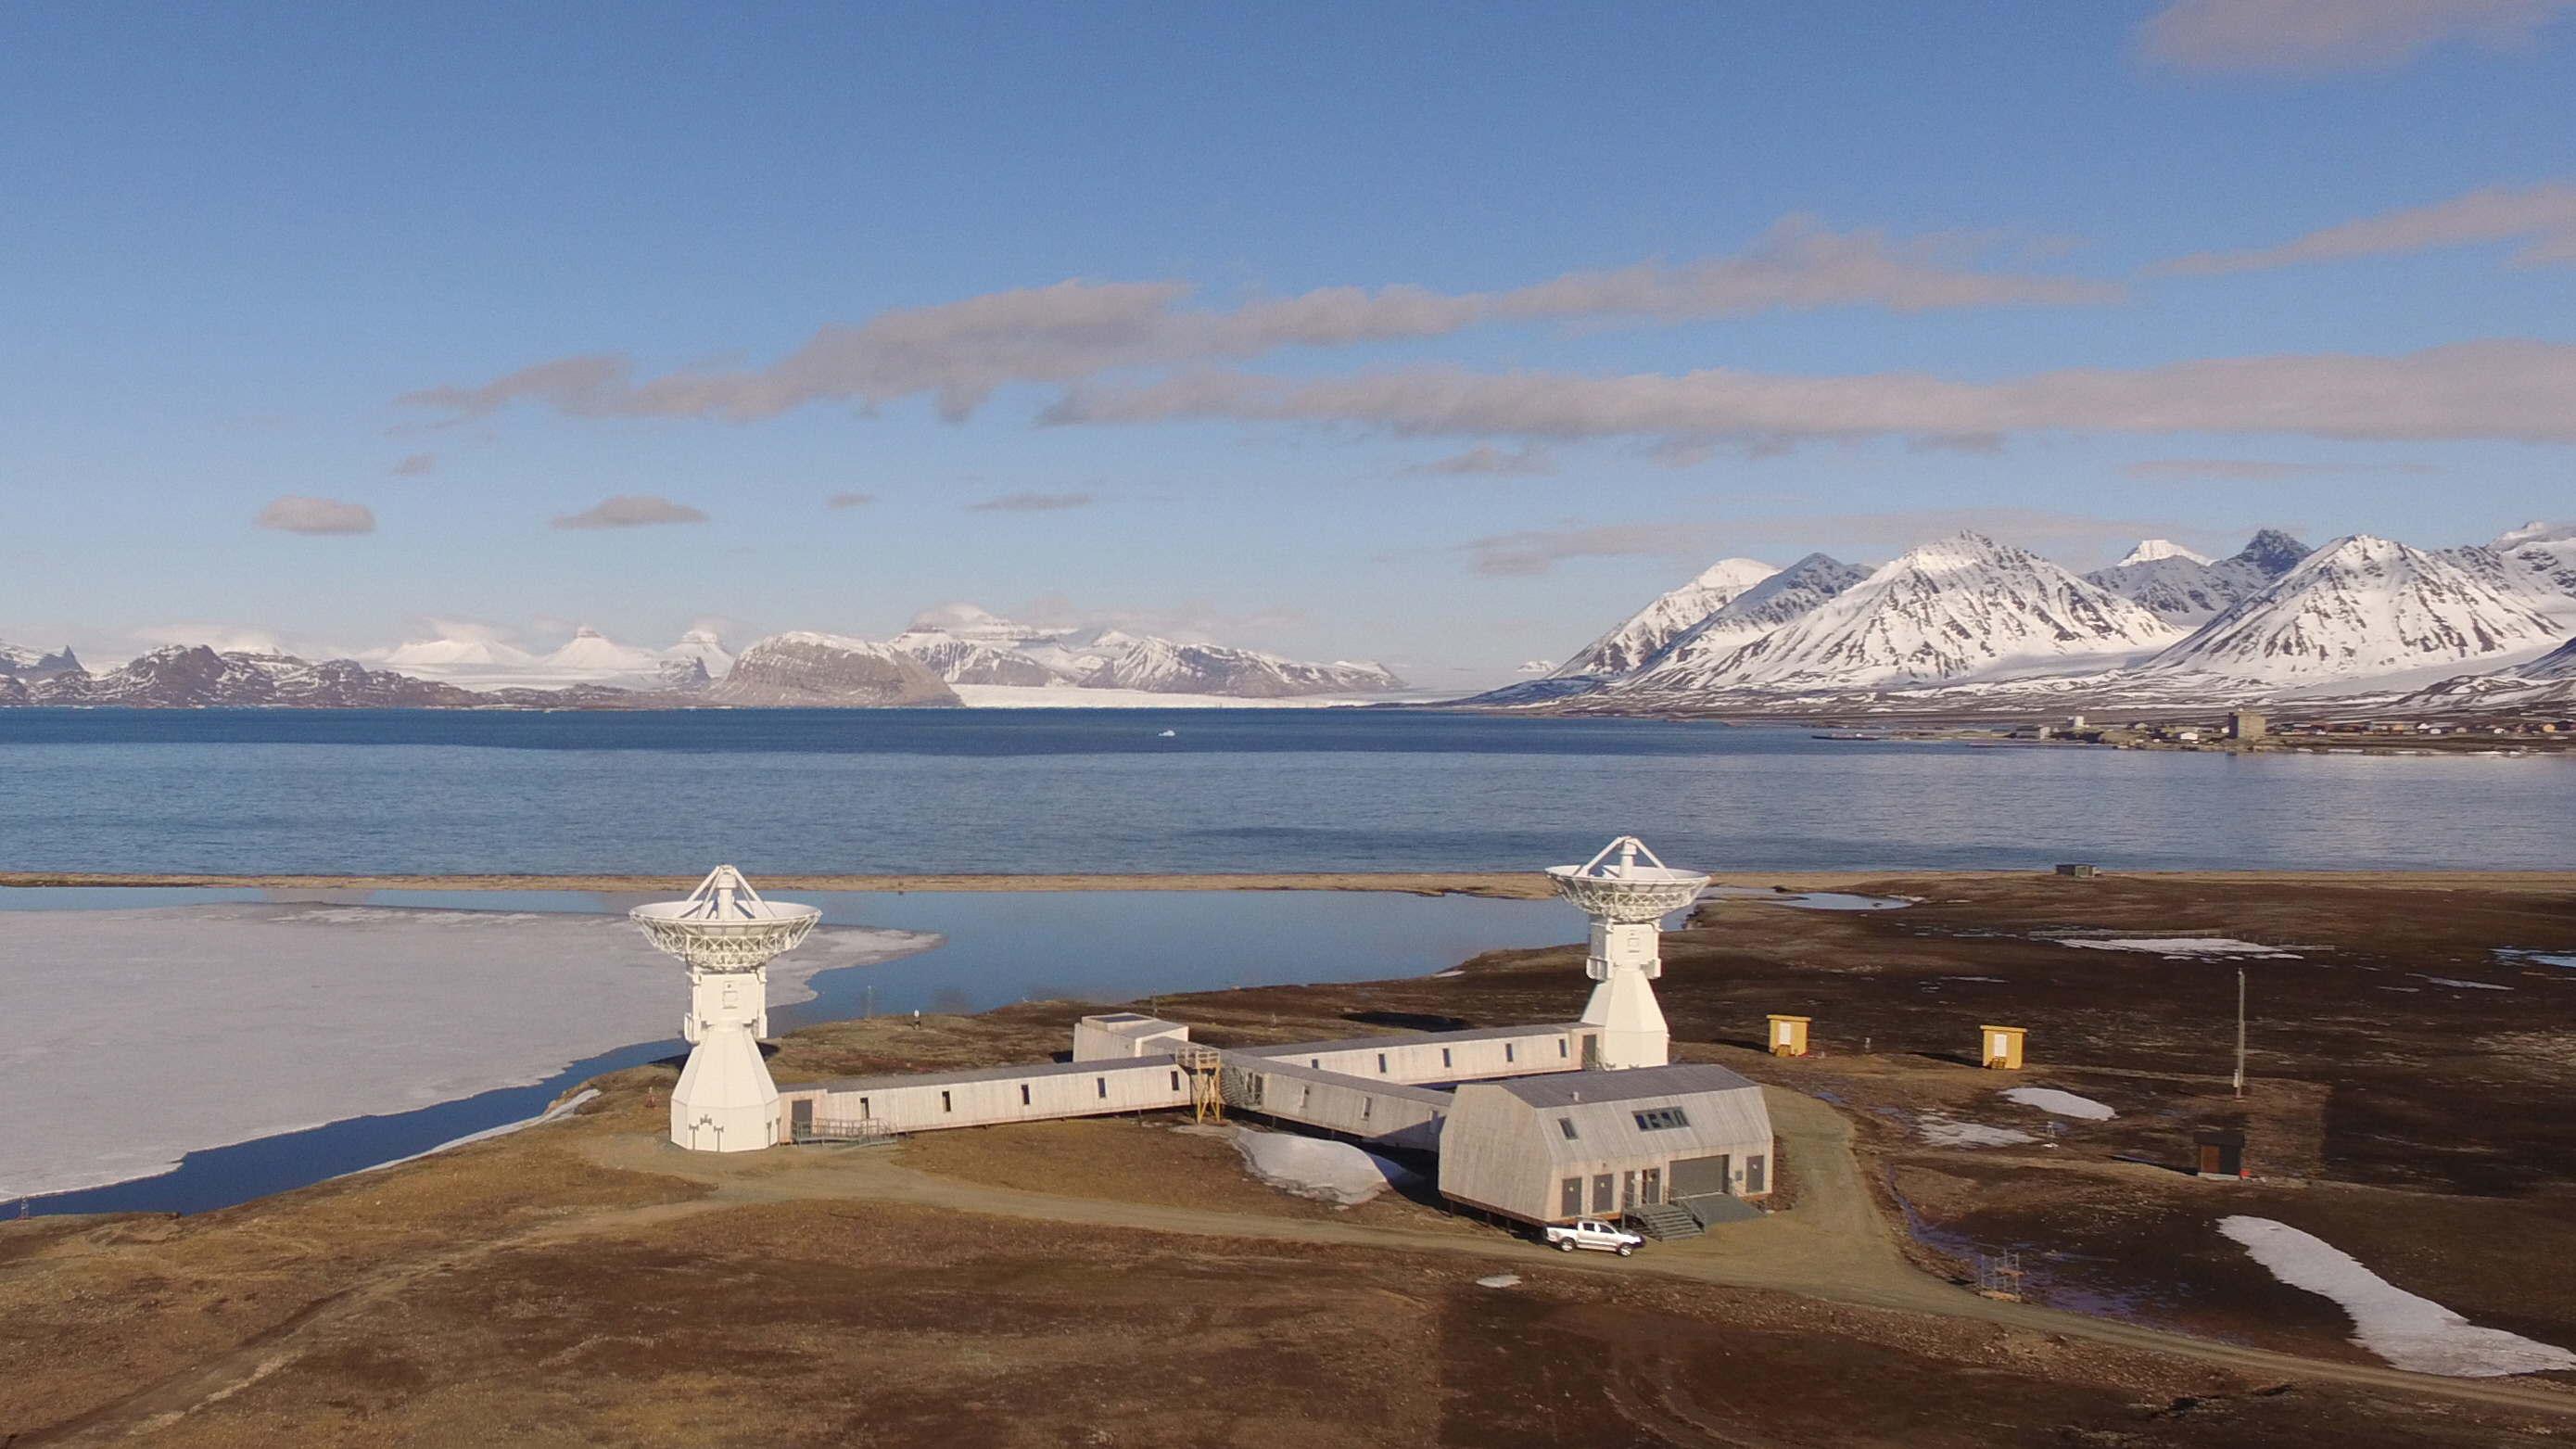
\includegraphics[width=0.9\textwidth]{figure/PAB_jordobservatoriet.jpg}\caption{Foto: Per Anders Bjørklund}
  \end{figure}
\end{frame}


\begin{frame}{Banen til LAGEOS-1}
  \begin{figure}
    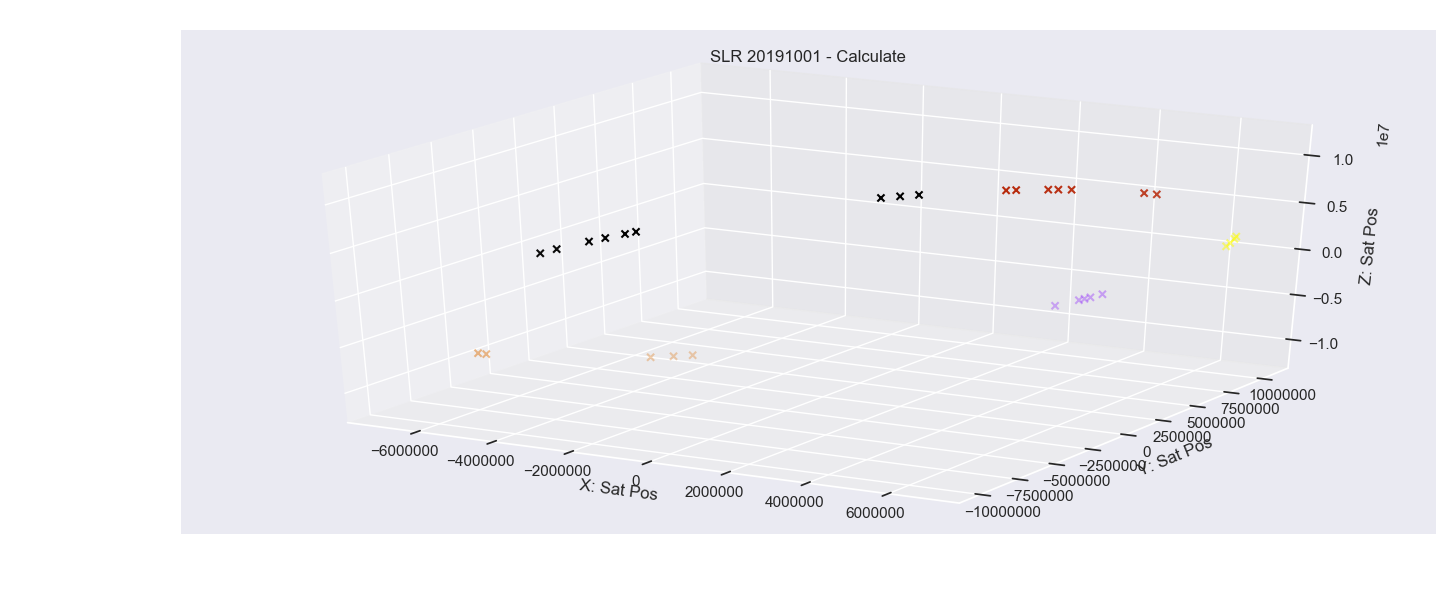
\includegraphics[width=0.9\textwidth]{figure/orbit_l1_4h.png}\caption{Bare 5 stasjoner målte mot Lageos1 i første omløp 1. oktober 2019. Banen er beregnet med {\it Where}.}
  \end{figure}
\end{frame}


\begin{frame}{Banen til LAGEOS-1}
  \begin{figure}
    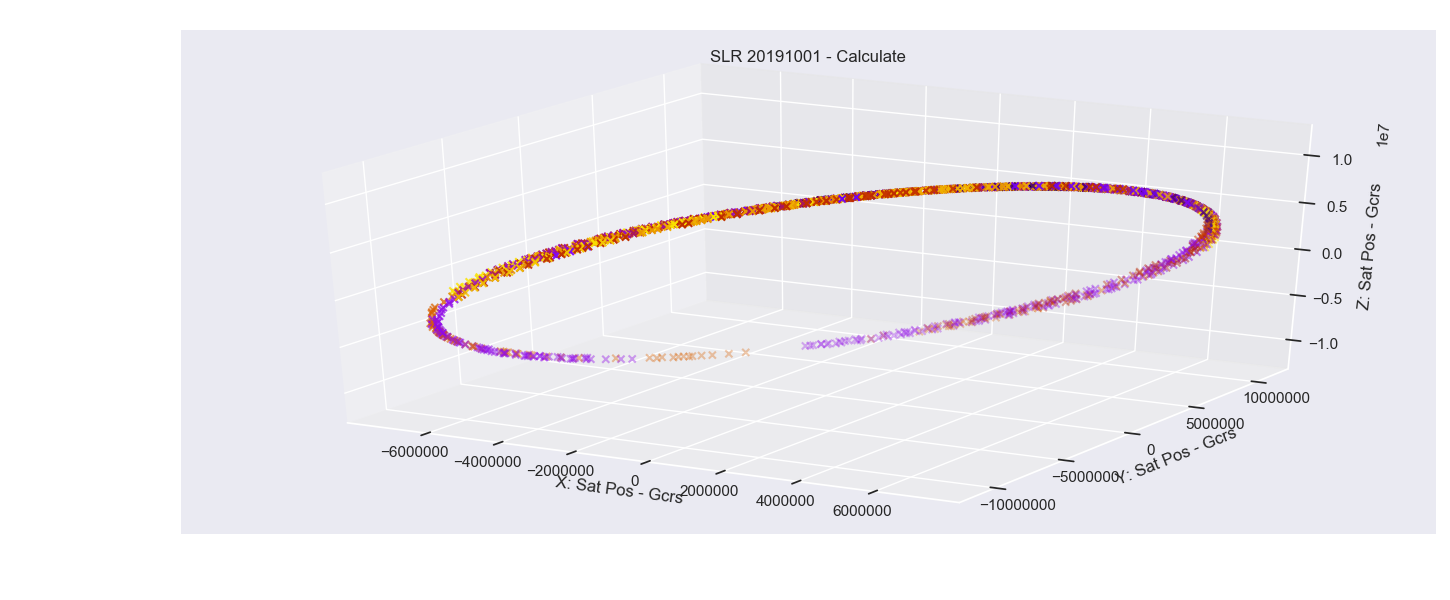
\includegraphics[width=0.9\textwidth]{figure/orbit_l1_week.png}\caption{26 stasjoner målte mot Lageos1 i perioden 1. - 7. oktober 2019. Banen er beregnet med {\it Where}.}
  \end{figure}
\end{frame}


\begin{frame}{ITRF}
\framesubtitle{International Terrestrial Reference Frame}
  \begin{description}
    \item[Hvorfor?] For å kunne måle platetektonikk, havnivå masseforflytninger etc. i referanse til noe
    \item[Hvordan?] Laget ved hjelp av fire geodetiske teknikker GPS, VLBI, SLR og DORIS
    \item[Når?] Må oppdateres jevnlig, fordi vi har nye modeller, nytt måleutstyr, og fordi jorda forandrer seg
    \item[Sist gang:] ITRF2014
    \item[Neste gang:] ITRF2020
  \end{description}
\end{frame}


\begin{frame}{Referanserammen}
  \begin{columns}
    \column{0.22\textwidth}
      \vspace{0.9cm}
      \begin{figure}
        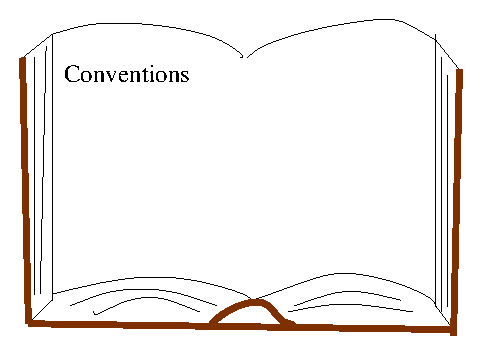
\includegraphics[width=0.95\textwidth]{figure/book.eps}\caption{Regelboken}
      \end{figure}
    \column{0.08\textwidth}\\ \ \\ \ \\ \ \\ \ \\ 
      +  
    \column{0.22\textwidth}
      \begin{figure}
        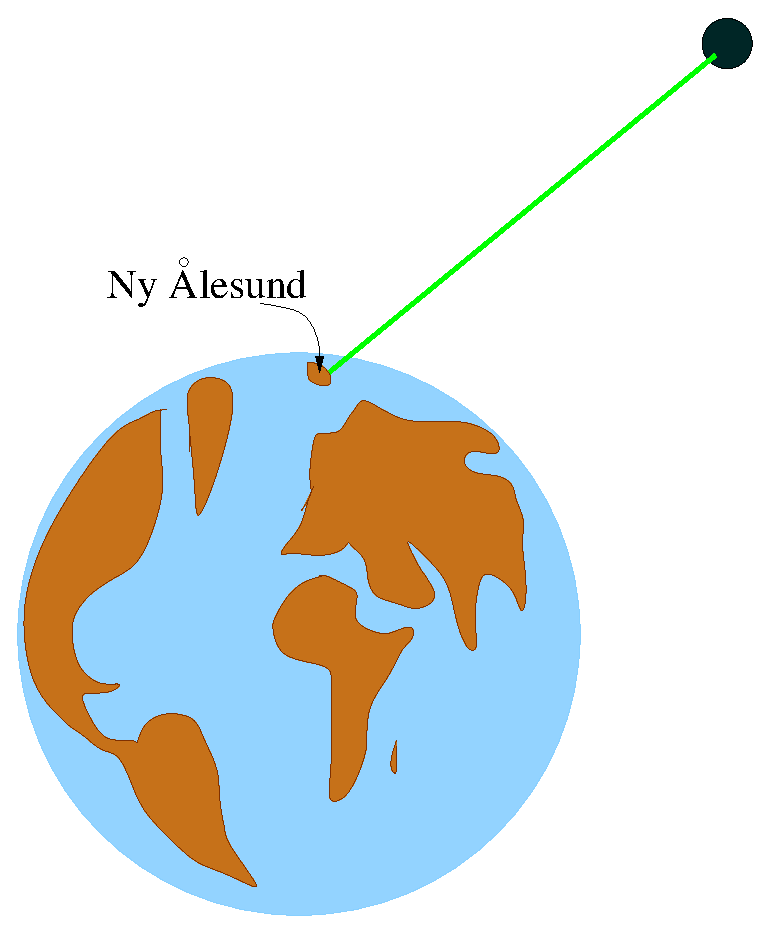
\includegraphics[width=0.95\textwidth]{figure/jordklode.eps}\caption{Observasjoner}
      \end{figure}
    \column{0.08\textwidth}\\ \ \\ \ \\ \ \\ \ \\
      =
    \column{0.26\textwidth}
      \\ \ \\ 
      \begin{figure}
        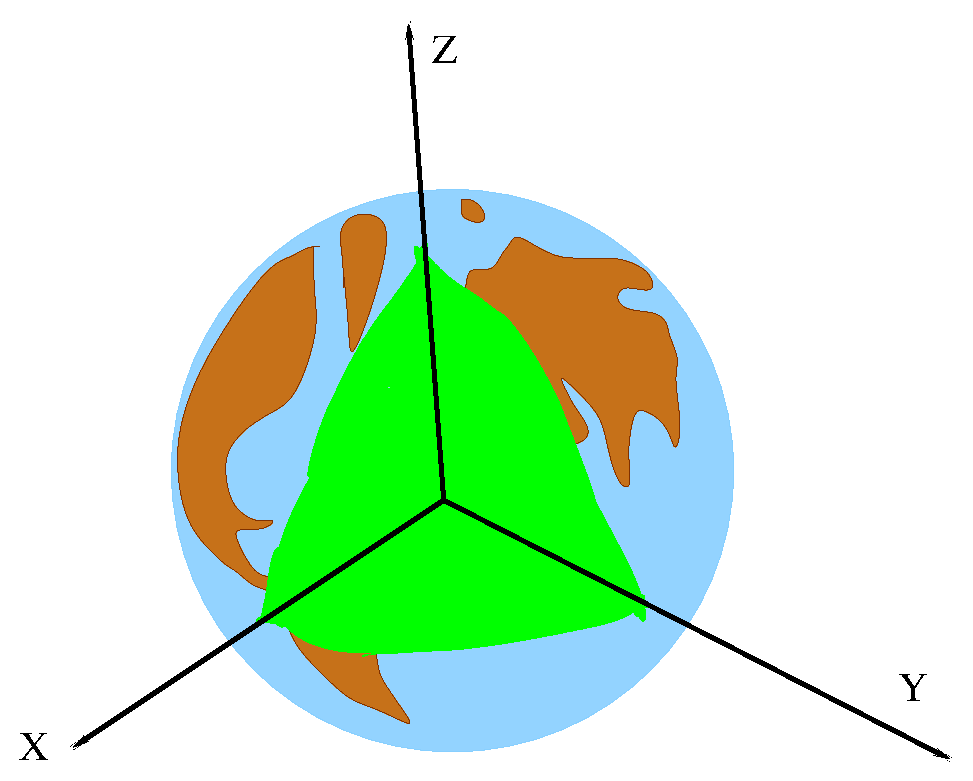
\includegraphics[width=0.97\textwidth]{figure/referanseramme.eps}\caption{Referanserammen}
      \end{figure}
  \end{columns}
\end{frame}


\begin{frame}{Jordrotasjonsparametre}
  \begin{center}
    \begin{figure}
      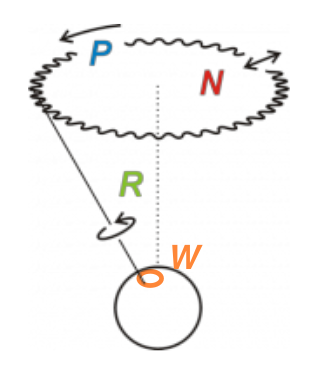
\includegraphics[width=0.15\textwidth]{figure/eop_parameters.png}
    \end{figure}

  \begin{figure}
    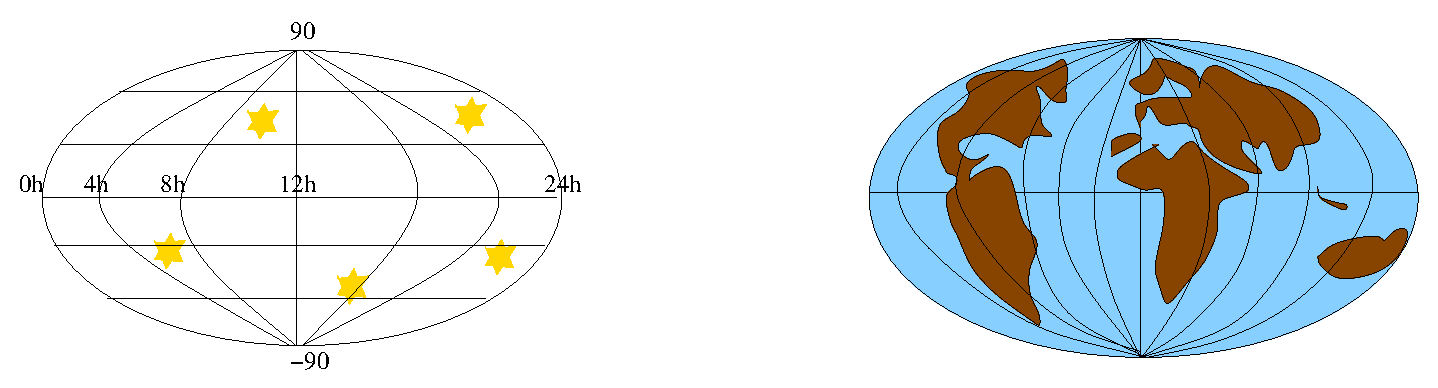
\includegraphics[width=0.8\textwidth]{figure/eop.eps}\caption{Hvordan jordfast system er rotert i forhold til himmelfast system.}
  \end{figure}
  \end{center}
\end{frame}


\begin{frame}{Verdikjeden for SLR}
\framesubtitle{(og hvor Kartverket vil være med og bidra i fremtiden)}
  \begin{tabular}{clc}
    &  \\
    \fbox{40+ stasjoner med SLR} & 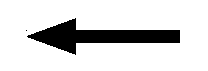
\includegraphics[width=0.08\textwidth]{figure/pil_horisontal.eps}  & \fbox{
          
\includegraphics[width=0.1\textwidth]{figure/kartverket.png}}\\

    
\includegraphics[width=0.015\textwidth]{figure/pil.eps} && \\

    \fbox{2 datasentre i USA/Tyskland} && \\

    
\includegraphics[width=0.015\textwidth]{figure/pil.eps} && \\
    \fbox{7 analysesentre} & 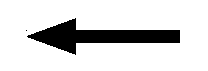
\includegraphics[width=0.08\textwidth]{figure/pil_horisontal.eps} &  \fbox{
          
\includegraphics[width=0.1\textwidth]{figure/kartverket.png}}\\

    
\includegraphics[width=0.015\textwidth]{figure/pil.eps} && \\
    \fbox{2 kombinasjonssentre i USA/Italia} & &\\
  \end{tabular}
\end{frame}


\begin{frame}{Verdikjeden for referanserammen}
\framesubtitle{International Earth Rotation and Reference Systems Service (IERS) koordinerer arbeidet}
  \begin{tabular}{clc}
    &  \\
    \fbox{VLBI + SLR + GNSS + DORIS + Local Ties} \\

    
\includegraphics[width=0.015\textwidth]{figure/pil.eps} \\

    \fbox{Kombinasjon i Tyskland/Frankrike/USA} \\

    
\includegraphics[width=0.015\textwidth]{figure/pil.eps} \\

    \fbox{ITRF: International Terrestrial Reference Frame}

  \end{tabular}
\end{frame}


\begin{frame}{Korreksjoner}
  \begin{itemize}
    \item Betyr ikke at målingen er «feil»
    \item I SLR måler vi gangtiden til signalet, ikke faktisk avstand
    \item Forsinkelse av signalet gjennom atmosfæren utgjør 3-4 meter
    \item Signalet reflekteres ikke i sentrum av satellitten
    \item Stasjonsforflytning: Tidekrefter etc.
  \end{itemize}
\end{frame}


\begin{frame}{Baneberegning}
  \begin{itemize}
    \item Analysesentrene beregner sine egne baner
    \item Iterativ prosess, numerisk integrasjon
    \item Må ta hensyn til alle krefter som virker på satellitten
    \item Minste kvadraters metode tilpasning til målingene
    \item Bruker banen som en «fast referanse i rommet», regner ut korreksjoner for stasjonsposisjonene etterpå
  \end{itemize}
\end{frame}


\begin{frame}{Where}
  \framesubtitle{Vår programvare for geodetisk analyse}
  \begin{itemize}
    \item Utvikles ved Kartverket
    \item Skrives i Python
    \item Testleveranser til International VLBI Service pågår
    \item Plan om testleveranser også til International Laser Ranging Service i løpet av 2020
    \item Har som målsetning å bli analysesenter for VLBI og SLR
  \end{itemize}
  \begin{center}
    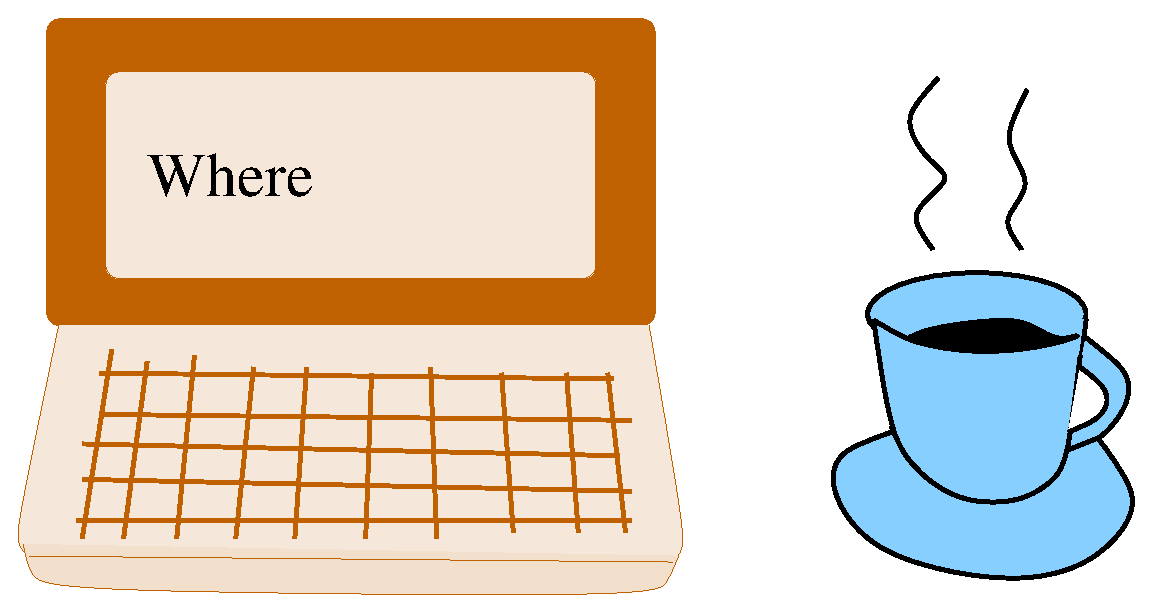
\includegraphics[width=0.3\textwidth]{figure/where.eps}
  \end{center}
\end{frame}

\end{document}
}
          \end{block}
        \end{column}
        \begin{column}{.22\textwidth}
          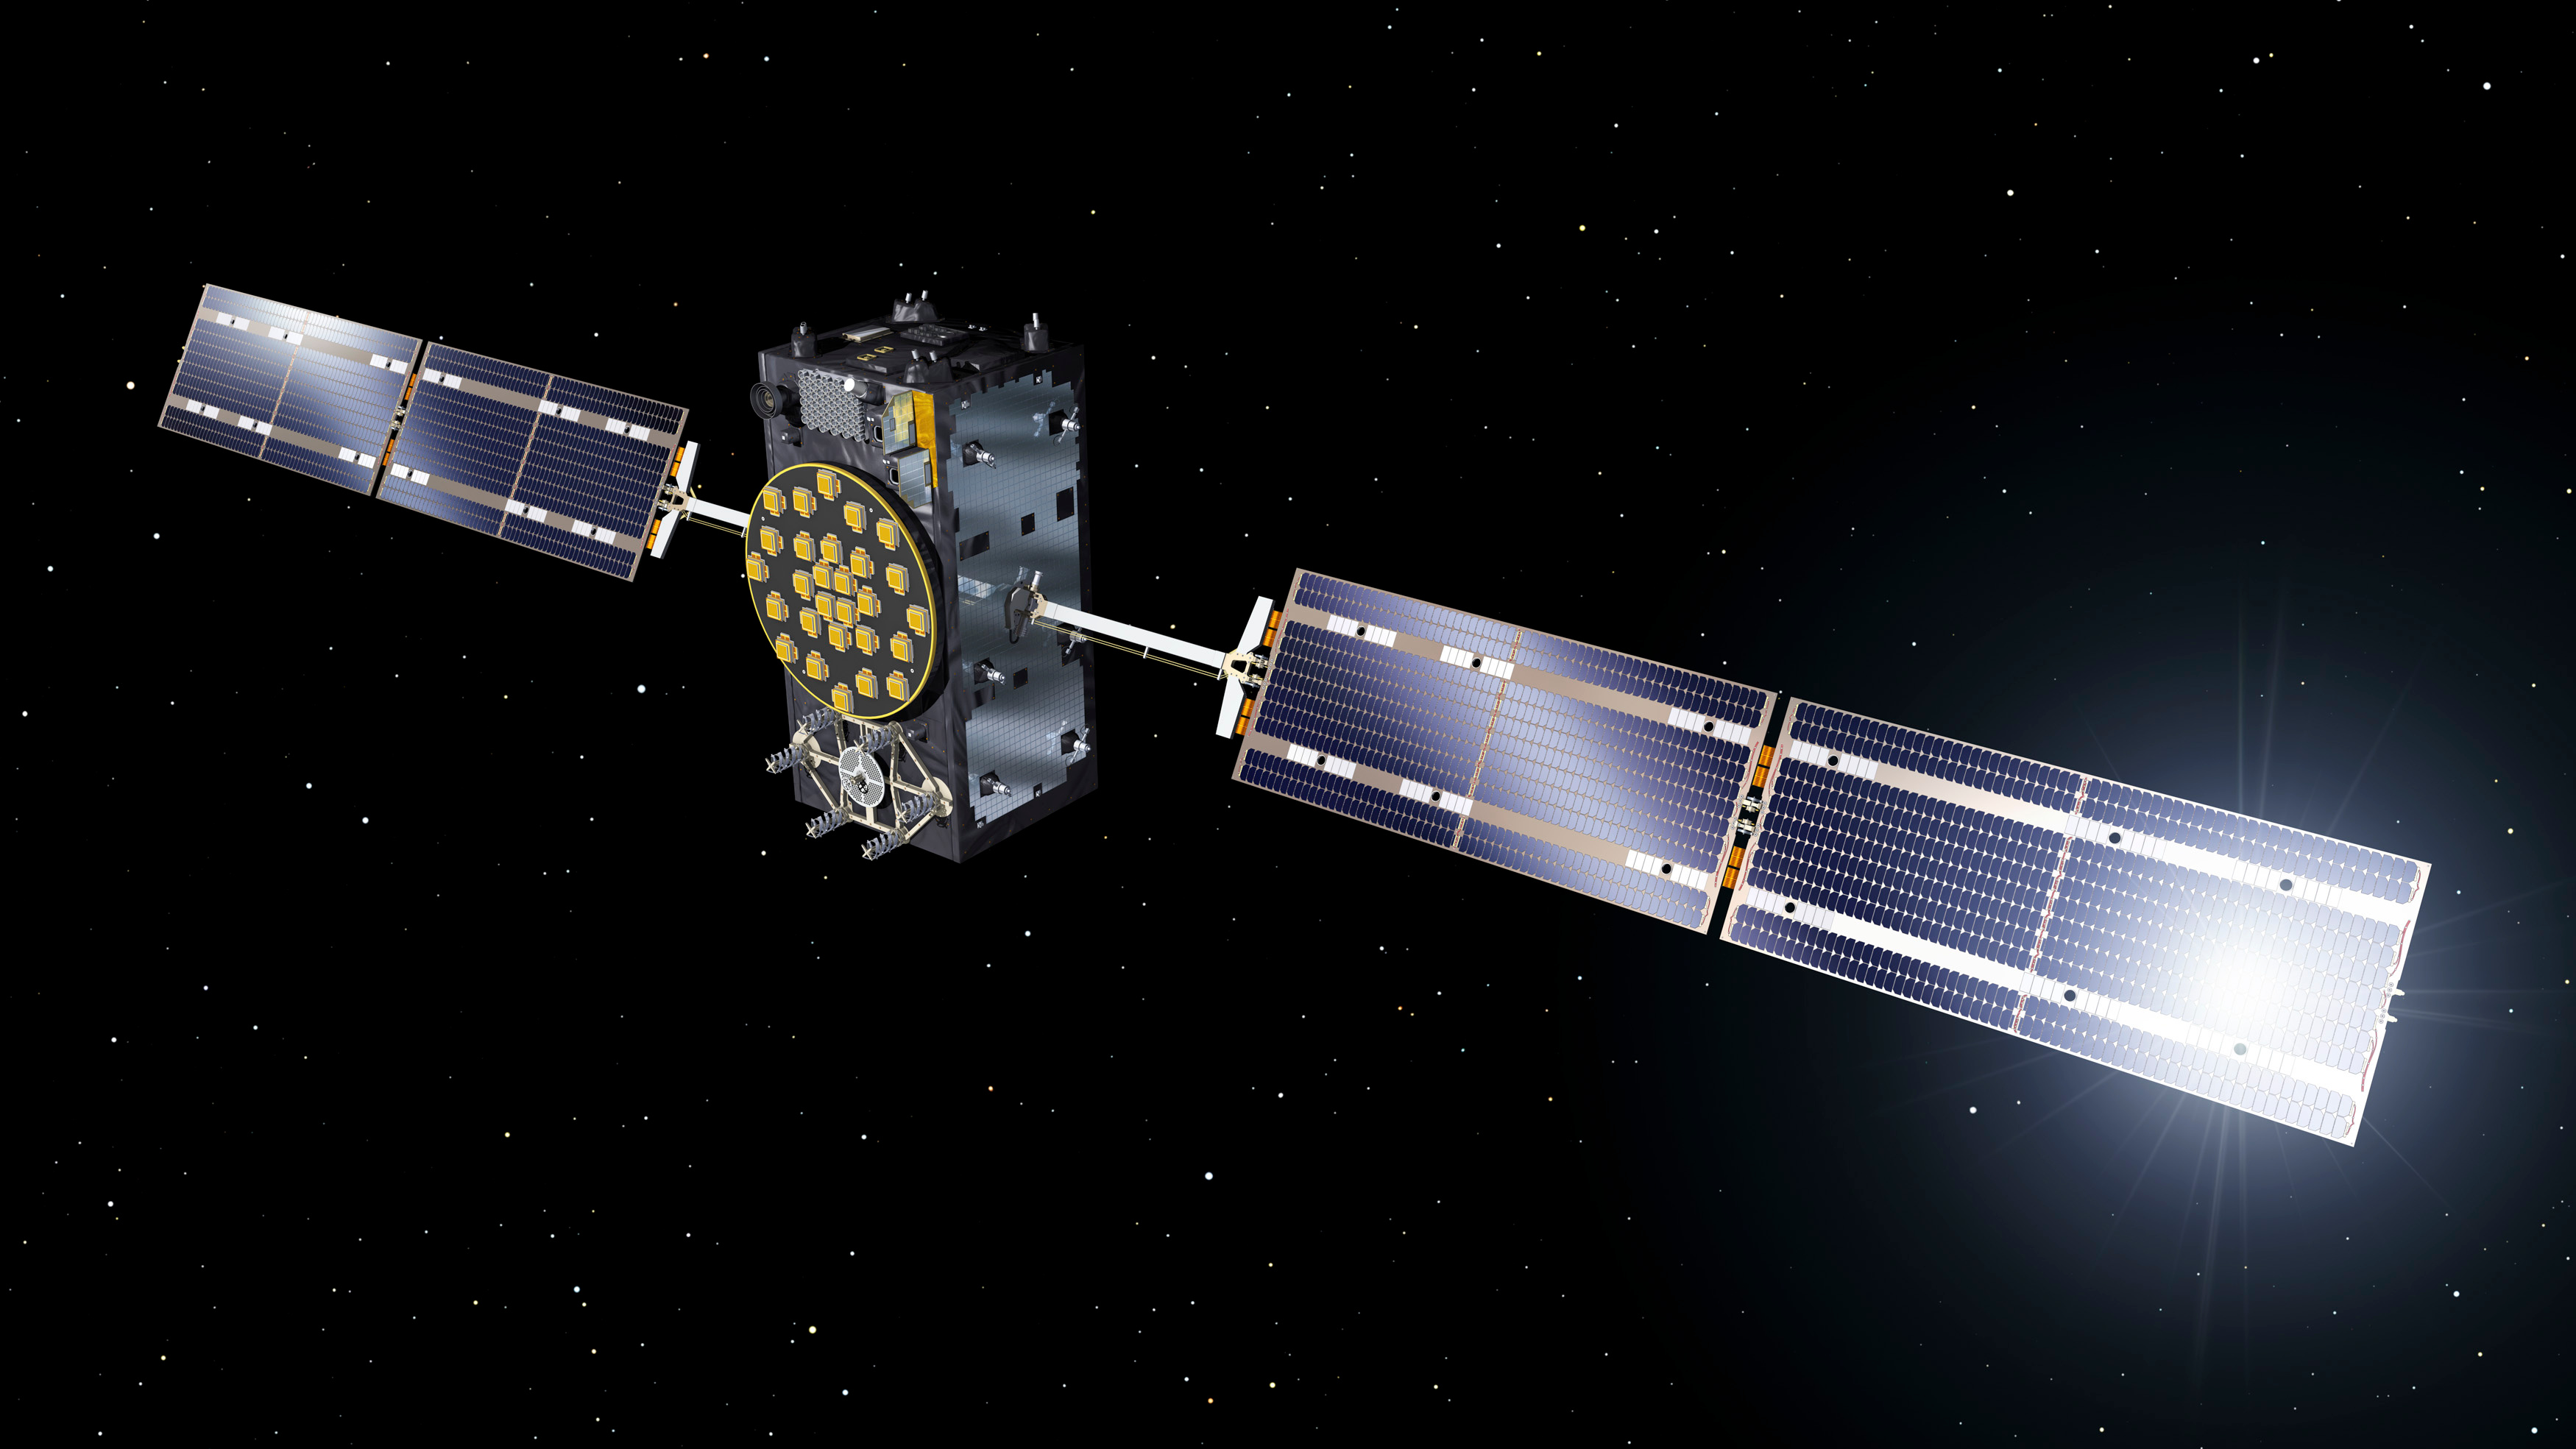
\includegraphics[width=\textwidth]{figure/gnss}
          \raisebox{10cm}{\kern-5cm\color{white}\tiny
            PHOTO: ESA -- J. HUART}
          \vskip-1ex
          \begin{block}{GNSS}
            \vskip-3ex
            \parbox[t][\techheight]{0.95\textwidth}{\raggedrightGlobal Navigation Satellite Systems (GNSS) are networks of satellites used to accurately calculate positions on
Earth. Such systems include the American GPS, the Russian GLONASS and the European Galileo-system. They all work by
measuring the time a signal takes from the satellites to a receiver and calculating distances based on these.

\endinput
}
          \end{block}
        \end{column}
        \begin{column}{.22\textwidth}
          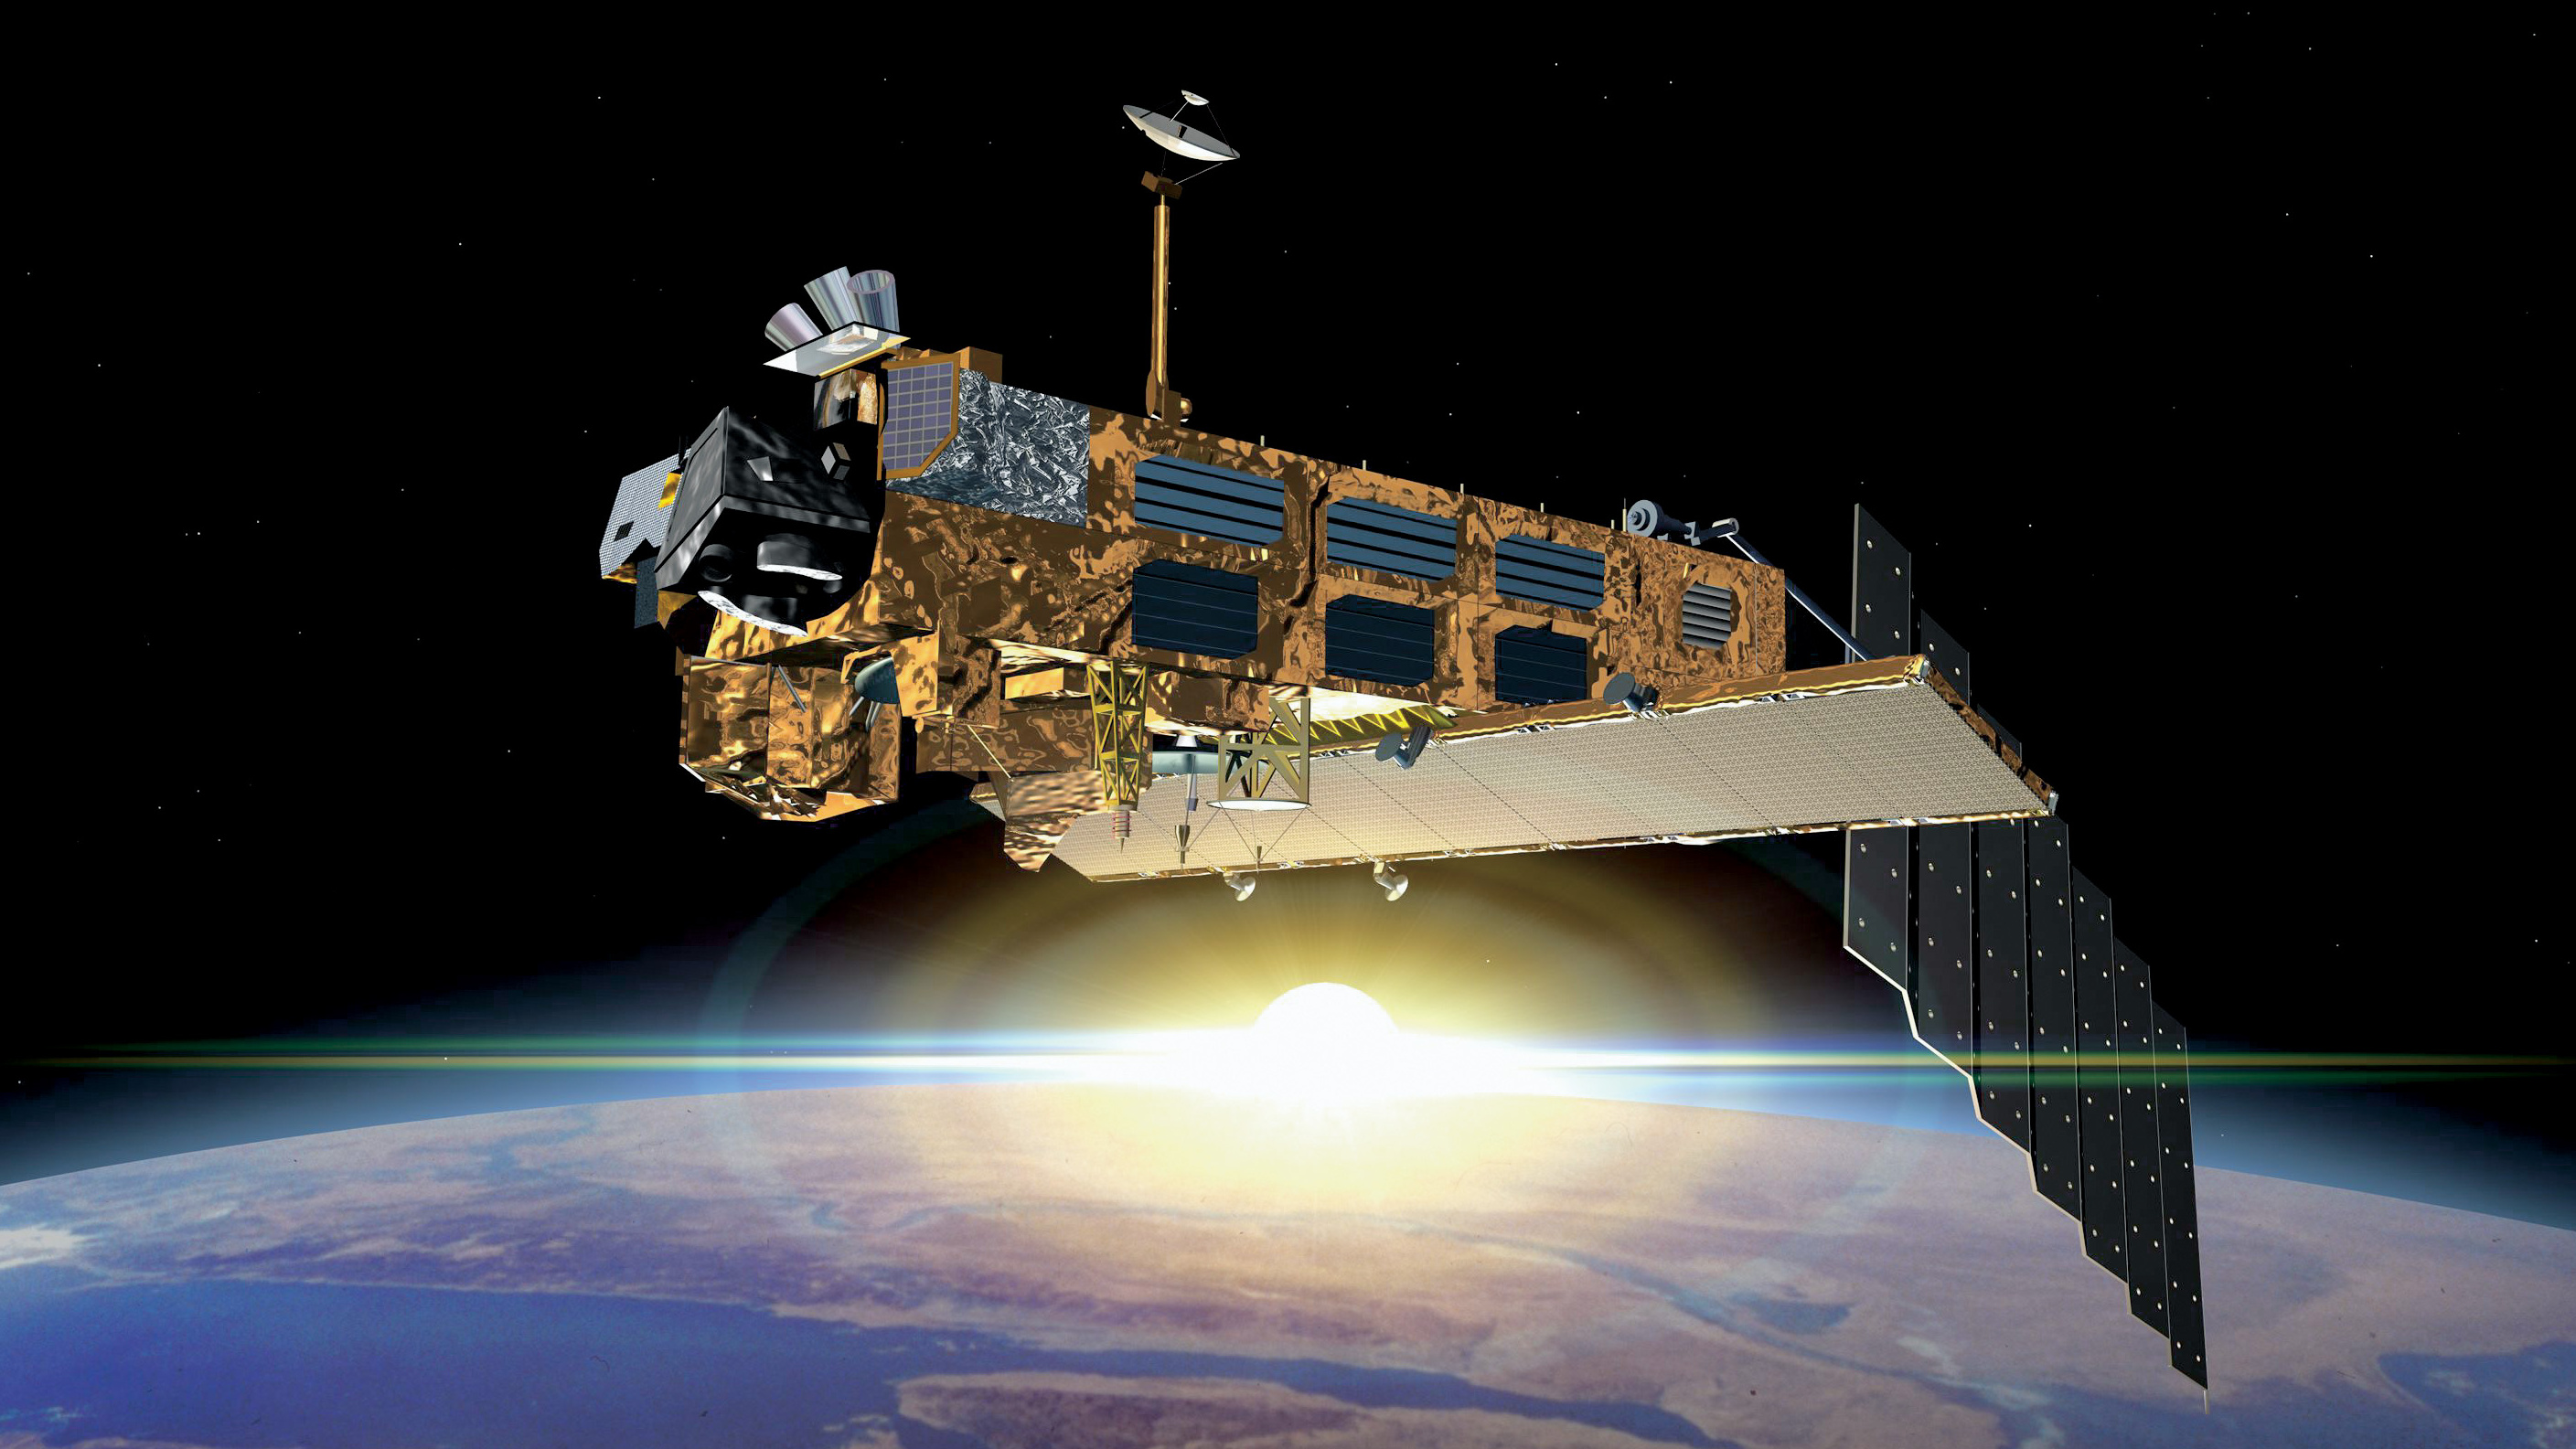
\includegraphics[width=\textwidth]{figure/doris}
          \raisebox{10cm}{\kern-8.3cm\color{white}\tiny
            PHOTO: ESA -- DENNMAN PRODUCTIONS}
          \vskip-1ex
          \begin{block}{DORIS}
            \vskip-3ex
            \parbox[t][\techheight]{0.95\textwidth}{\raggedrightDoppler Orbitography and Radiopositioning Integrated by Satellite (DORIS) is a
system consisting of a network of ground-based beacons emitting signals that are
picked up by satellites as they fly by. Satellite orbits and beacon positions
can be calculated based on the Doppler effect, the frequency shift of the beacon
signal caused by the satellite movement.

\endinput
}
          \end{block}
        \end{column}
      \end{columns}
      
      \vspace*{3cm}

      \begin{columns}
        \begin{column}[t]{.72\textwidth}
          \begin{block}{Combination}
            \begin{multicols}{3}
              GEOSAT combines VLBI, SLR, GNSS, and DORIS data at the observation level as follows.

First, a 24h data set (an arc) (SLR: 1 week) is sorted in batches of
passes (FIGURE 1) for each geodetic technique. A pass is defined by observing a specific radio source or satellite from one or several specific ground or satellite based receivers. A transition from one pass to the next is defined
by a switch of one or more objects that are involved in the
computation of the residual. For instance, for VLBI the objects are
two stations and one radio source, for SLR the objects are one station
and one satellite. Each pass has its own copy of the state vector so
that it is possible to re-estimate all or parts of the state vector
for each pass as part of the next step: reducing the residuals by
least-squares estimation of some subset of 
parameters (clock, troposphere, range biases, ...). However, by increasing the state vector dimension it is
also possible to allow parameters to have an impact on the calculated
observations for time spans that are not restricted by the length of a
pass.

In the residual reduction step, in which the different observation techniques
are treated separately, outliers are removed and the impact of
discontinuities like VLBI clock breaks on the residuals are
reduced. This is essential for the next computation step in which the
techniques are combined sequentially, observation epoch by observation
epoch, by a UD (Upper Diagonal) Kalman filter. Especially, since sequential filters are more
susceptible to outliers than batch algorithms.

In the combination step it is important to note that the full state
vector and its a posteriori variance-covariance matrix are updated at
each epoch according to the postulated observation noise. In this way
information from one technique can resolve the parameter correlations
of a different technique in a natural way since these are described by
the full variance-covariance matrix. For instance, if we truncate the a posteriori variance-covariance matrix for each technique separately (for instance VLBI or SLR) before combination,
then important technique specific correlations, and therefore
information on the weaknesses of the individual solutions, could be lost. These
weaknessess of the solution are commonly re-established by applying a
Helmert type transformation to it before combination with other data
types.

As a first approach we will combine SLR and VLBI data so that the only parameters that
are shared by both techniques are Earth Rotation Parameters. However, in order to exploit that we
account for all correlations while combining the data types epoch by epoch it is possible that we
need a stronger connection between SLR and VLBI. Therefore we consider
implementing local ties at collocation sites as the first observation
in all data sets. An issue here will be, when added as
constraints in all data sets, and not only once as they should, the effective constraint imposed by the local
ties will be unrealistically strong.

When the sequential processing of data from all techniques within the
specified data set ($N_\mathrm{e}$ epochs) is finished we are left with an a posteriori state
vector, which is derived without any neglectance
of parameter correlations. The end state vector will typically consist
of $N_\mathrm{g}$ global parameters that are constant across the data set, like
station coordinates, and $N_\mathrm{s}$ stochastic parameters, describing the
troposphere or clock model errors, at the last epoch. Ideally, we
would then have backward filtered (smoothed) the state vector and
variance-covariance matrix to establish a larger matrix and state vector with dimension
\begin{equation}\nonumber
N=N_\mathrm{g}+N_\mathrm{s}\,N_\mathrm{e},
\end{equation}
formally containing all available information. However, using the complete variance-covariance information in the combination of data sets (arcs) (FIGURE 2), to obtain solutions spanning years,
is not feasible since the effective state vector will contain millions $\sim{}N_\mathrm{s}\,N_\mathrm{e}$ of parameters.

\endinput

            \end{multicols}
          \end{block}

          \begin{columns}
            \begin{column}{.65\textwidth}
              \begin{figure}
                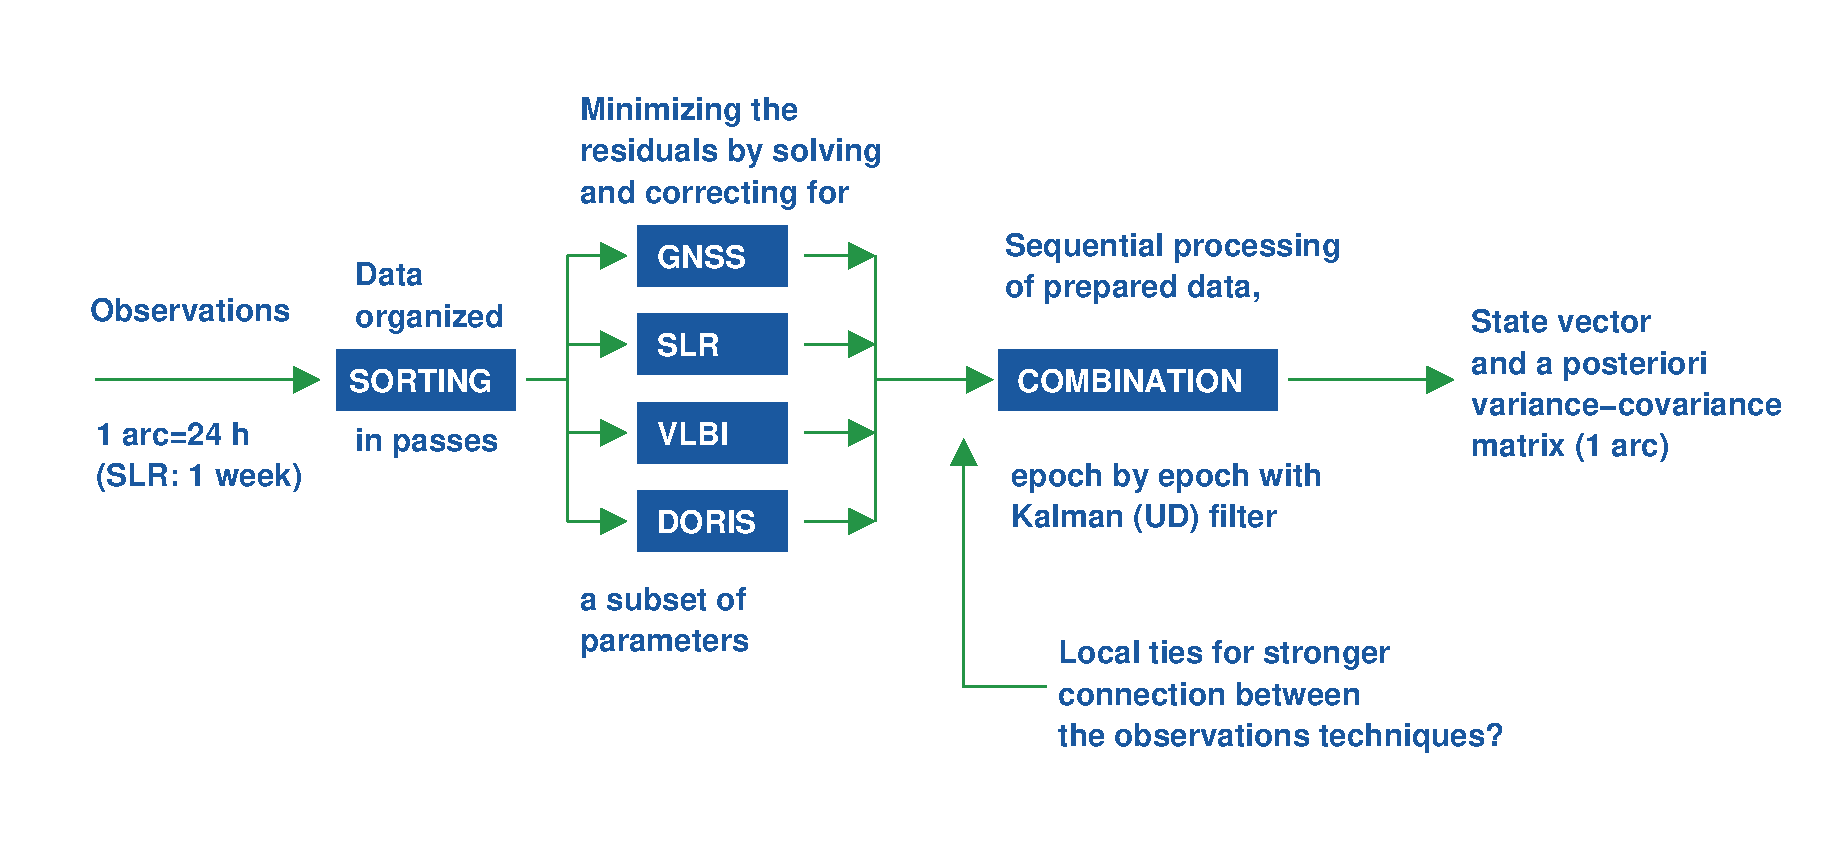
\includegraphics{figure/flow}
                \caption{The flow chart for the processing of one data set is shown.}
              \end{figure}
            \end{column}
            \begin{column}{.3\textwidth}
              \begin{figure}
                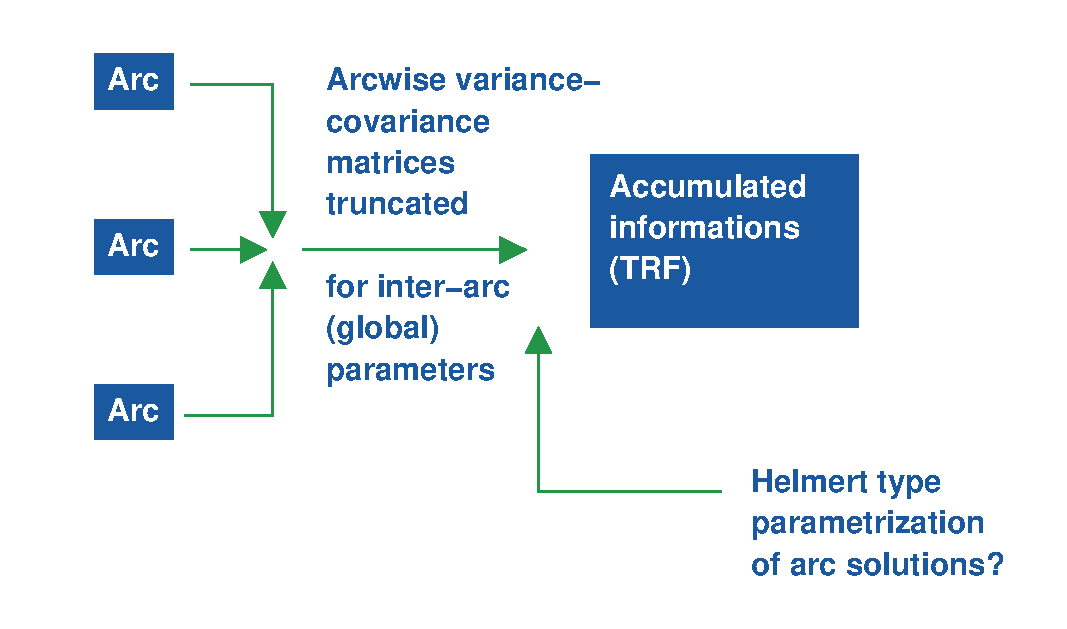
\includegraphics{figure/accum}
                \caption{An overview on how the data sets will be combined.}
              \end{figure}
            \end{column}
          \end{columns}
        \end{column}
        \begin{column}[t]{.22\textwidth}
          \begin{block}{Future}
%            \begin{multicols}{1}
              At the moment we work on challenges connected to the combination of VLBI and SLR epoch by epoch. One important issue in this respect will be how we tie the VLBI and SLR network together. For instance, it will be important that the networks are closely connected at an early stage (during epoch by epoch processing with UD Kalman filter) so that the techniques may fully complement each other, before we truncate the state vector and its variance-covariance matrix for the accumulated combination solution. To what extent will the Earth Rotation Parameters, shared by both techniques, connect the different networks and, alternatively, how will we use local ties? Shall we use all available local ties, or only the most reliable?

The output of each data set will be a state vector consisting of global (station coordinates) and stochastic parameters (clock, troposphere) at the last epoch of the data set. Although no approximations regarding correlations have been made at this stage, the solution's a posteriori variance-covariance matrix does not contain all available information on parameter correlations. If we use only this limited information (state and covariance at last epoch), as we intend to due to practical reasons (see Combination), it is possible that we during day by day combination have to involve Helmert transformations to describe the weaknesses of daily solutions.       

In the future we will include GNSS and DORIS in our processing chain, which we anticipate will require the introduction of new parameter types to achieve intra-technique consistency.    


\endinput

%            \end{multicols}
          \end{block}
        \end{column}
      \end{columns}
    \end{column}
  \end{columns}
\end{frame}
\end{document}
